\documentclass[onecolumn, 12pt]{book}

\usepackage[latin1]{inputenc}   
\usepackage{amsmath}
\usepackage{algorithm}
\usepackage{algorithmic} 
%\usepackage[T1]{fontenc}

%\usepackage[francais]{babel}     
\usepackage{layout}    
\usepackage[top=2cm, bottom=2cm, left=2cm, right=2cm]{geometry} 
\usepackage{setspace}
\usepackage{soul}
\usepackage{color} 
\usepackage{verbatim}
\usepackage{moreverb}
\usepackage{listings}
\usepackage{url}
\usepackage{graphicx}
\usepackage{epstopdf}
\usepackage{caption}
\usepackage{setspace}
 
 
% \title{Mod\`ele de Donn\'ees}
% \author{Willy Ehounou}
 %\date{01/06/15}
\title{Plan de th\`ese}
%\author{Jules \bsc{Verne}}
\date{\oldstylenums{1875}} 


 
\begin{document}
\maketitle
\tableofcontents

\chapter{Simulation des algorithmes sur r\'eseaux th\'eoriques}

\section{Objectifs}
Le but des simulations faites ci-dessous est de montrer que le graphe produit par les algorithmes (couverture et correction) est le plus proche du graphe r\'eel quand la matrice de corr\'elation associ\'ee au graphe r\'eel presente peu d'erreurs de corr\'elation.
Une erreur de corr\'elation est l'existence d'une corr\'elation entre deux arcs (ajout de $1$ dans la matrice) lorsqu'il n'en existe pas. De m\^eme, l'absence de corr\'elation entre 2 arcs (ajout de $0$ dans la matrice) lorsqu'il en existe  est aussi une erreur de corr\'elation.


\section{D\'efinition de la m\'etrique: distance de Hamming}
La m\'etrique utilis\'ee pour diff\'erencier deux graphes est la {\em distance de Hamming}.
La distance de Hamming est le rapport du nombre d'ar\^etes diff\'erentes dans le graphe produit (en comparaison avec le graphe r\'eel) sur le nombre total d'ar\^etes dans le graphe r\'eel.
On consid\`ere deux types d'ar\^etes diff\'erentes:
\begin{itemize}
	\item Les ar\^etes dans le graphe produit inexistante dans le graphe r\'eel. Elles correspondent \`a $1$ dans la matrice du graphe produit et \`a $0$ dans la matrice du graphe r\'eel. 
	\item Les ar\^etes dans le graphe r\'eel inexistante dans le graphe produit. Elles correspondent \`a $1$ dans la matrice du graphe r\'eel et \`a $0$ dans la matrice du graphe produit. 
\end{itemize} 
Ainsi, une distance de Hamming \'egale \`a $0$ signifie que le graphe produit est le graphe r\'eel tandis que  une distance de Hamming superieure ou \'egale \`a $1$ signifie que les graphes r\'eel et produit ne sont pas isomorphes en ar\^etes. 


\section{G\'en\'eration de graphes orient\'es}
La structure de donn\'ees utilis\'ee pour le graphe est une {\em matrice d'adjacence}.
La matrice d'adjacence est une matrice creuse carr\'ee de {\em n} sommets.
On d\'efinit manuellement le nombre de sommets {\em n} et le degr\'e moyen  $\alpha$ du graphe. 
La probabilit\'e d'existence d'une ar\^ete est de $p = \frac{\alpha}{N}$.
Toutefois, si le graphe obtenu par la matrice d'adjacence n'est pas connexe, on choisit aleatoirement un sommet de chaque composante connexe et on ajoute une ar\^ete entre ces sommets.
\newline
% orientation
Pour orienter les ar\^etes, on choisit certains sommets comme \'etant des sources et on les marque puis on leur attribue un  num\'ero d'ordre qui est l'ordre de parcours des sommets ( soit un BFS).
\`A partir des sommets sources, on consid\`ere les sommets adjacents non marqu\'es des sources qu'on ajoute dans une {\em file}. On ajoute des arcs entre les sources et ces sommets adjacents, ensuite on marque les sommets adjacents et enfin on leur ajoute un num\'ero d'ordre. On reprend l'\'etape pr\'ec\'edente \`a partir des sommets en t\^ete de la file et on s'arr\^ete lorsque la file est vide.
S'il existe des sommets adjacents marqu\'es n'ayant aucuns arcs entre eux, alors on ajoute un arc du sommet de num\'ero d'ordre minimal vers le sommet de num\'ero d'ordre maximal.
Le graphe obtenu est alors un $DAG$.
\newline
% ajout flots sur chaque arc
L'ajout des flots sur chaque arc se fait par un parcours en largeur (BFS).
On d\'efinit les valeurs minimales et maximales des grandeurs physiques s\'electionn\'ees selon le r\'eseau \'energetique \`a mod\'eliser. \`A titre d'exemple, les valeurs choisies pour des grandeurs \'electriques sont: les intensit\'es $I = [150, 200 ]$, les tensions $U = [220, 250]$, les puissances $P = [ 33000, 62500]$. \newline
On debute par les sommets sources dont on g\'en\`ere une valeur aleatoire comprise dans l'un de ces intervalles. 
Chaque arc sortant du sommet source re\c coit  un flot \'egal \`a la somme des valeurs aleatoires sur les arcs entrants du sommet source multipli\'ee par le facteur $\epsilon$( d\'esignant les pertes joules) et divis\'ee par le degr\'e sortant de ce sommet si nous avons comme grandeurs les intensit\'es et les puissances.
Dans le cas de grandeurs comme les tensions, le flot de chaque arc sortant est la valeur aleatoire multipli\'ee par le facteur $\epsilon$. 
On propage les valeurs des grandeurs physiques jusqu'\`a ce qu'on arrive sur des sommets puits.
L'application de ces r\^egles de flots permettent de v\'erifier la {\em loi de conversation des noeuds}.


\section{processus de simulations}
On g\'en\`ere $500$ graphes de flots de $n = 30$ sommets ayant un degr\'e moyen $\alpha = 5$.
On g\'en\`ere \'egalement le line graph de ces graphes de flots dont la matrice d'adjacence ou corr\'elation est not\'ee $matE$.
Sur chaque line graph, on supprime $k = \{1,2,3,\cdots, 10\}$ ar\^etes et on note le matrice obtenu $matE_{k}$.
On applique les algorithmes de converture et de correction sur la matrice $matE_{k}$ et on compare le graphe r\'eel dont le matrice est  $matE$ et le graphe produit dont la matrice $matE_{k}$ a \'et\'e modifi\'ee par l'algorithme de correction si cette matrice n'\'etait pas un line graph. 
Les resultats de notre simulation sont present\'es sur la figure \ref{distanceHammingDLDH} .

\begin{centering} 
\begin{figure}[htb!] 
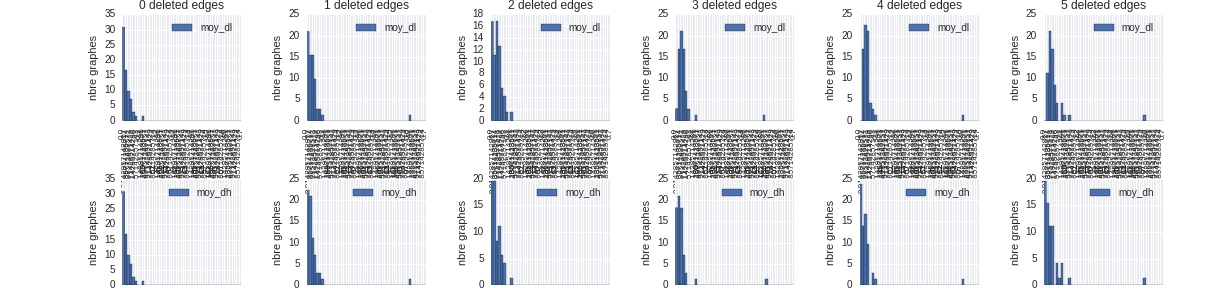
\includegraphics[scale=0.25]{/home/willy/Documents/courbePython/distanceMoyenDLDH.jpeg}
\caption{ distance line et de Hamming en fonction du nombre d'ar\^etes supprim\'ees }
\label{distanceHammingDLDH} 
\end{figure}
\end{centering} 

 
 
\section{R\'esultats}

\end{document}